\documentclass{beamer}
\mode<presentation>
\usepackage{xcolor}
\usepackage{amsmath}
\usepackage{amssymb}
%\usepackage{advdate}
\usepackage{adjustbox}
\usepackage{subcaption}
\usepackage{enumitem}
\usepackage{multicol}
\usepackage{mathtools}
\usepackage{listings}
\usepackage{url}
\usepackage[export]{adjustbox}
\def\UrlBreaks{\do\/\do-}
\usetheme{AnnArbor}
\usecolortheme{wolverine}
\setbeamertemplate{footline}

{
  \leavevmode%
  \hbox{%
  \begin{beamercolorbox}[wd=\paperwidth,ht=2.25ex,dp=1ex,right]{author in head/foot}%
    \insertframenumber{} / \inserttotalframenumber\hspace*{2ex} 
  \end{beamercolorbox}}%
  \vskip0pt%
}

 \usebackgroundtemplate{
\includegraphics[width=\paperwidth,height=\paperheight]{1.jpg}}

\begin{document}

\title{ASSIGNMENT 11}
\subtitle{Presentation On State Transition Diagram}

\author{Chetan Sarigala \\IIIT Raichur}
\date{\today}
\logo{
\includegraphics[height=1cm]{logo.png}}

\begin{frame}
\titlepage
\end{frame}

\AtBeginSection[]
{
\begin{frame}

\frametitle{Table of contents}
\tableofcontents[currentsection]
\end{frame}
}
\begin{document}

\section{Question}
\begin{frame}{Question}

%
.



The state transition diagram for the follwoing circuit is:
\begin{figure}[!ht]
\centerline{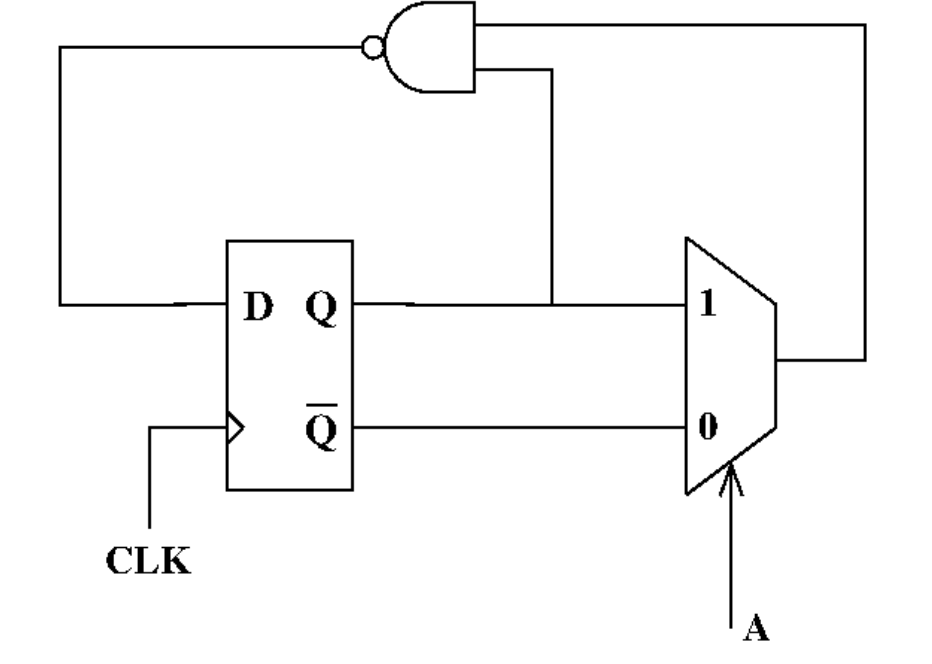
\includegraphics[scale=.6]{fig1.PNG}}
	
	\label{fig1.PNG}
\end{figure}
\end{frame}
%
\subsection{options}
\frametitle{options}
\begin{frame}{Options}
\begin{figure}[!ht]
\centerline{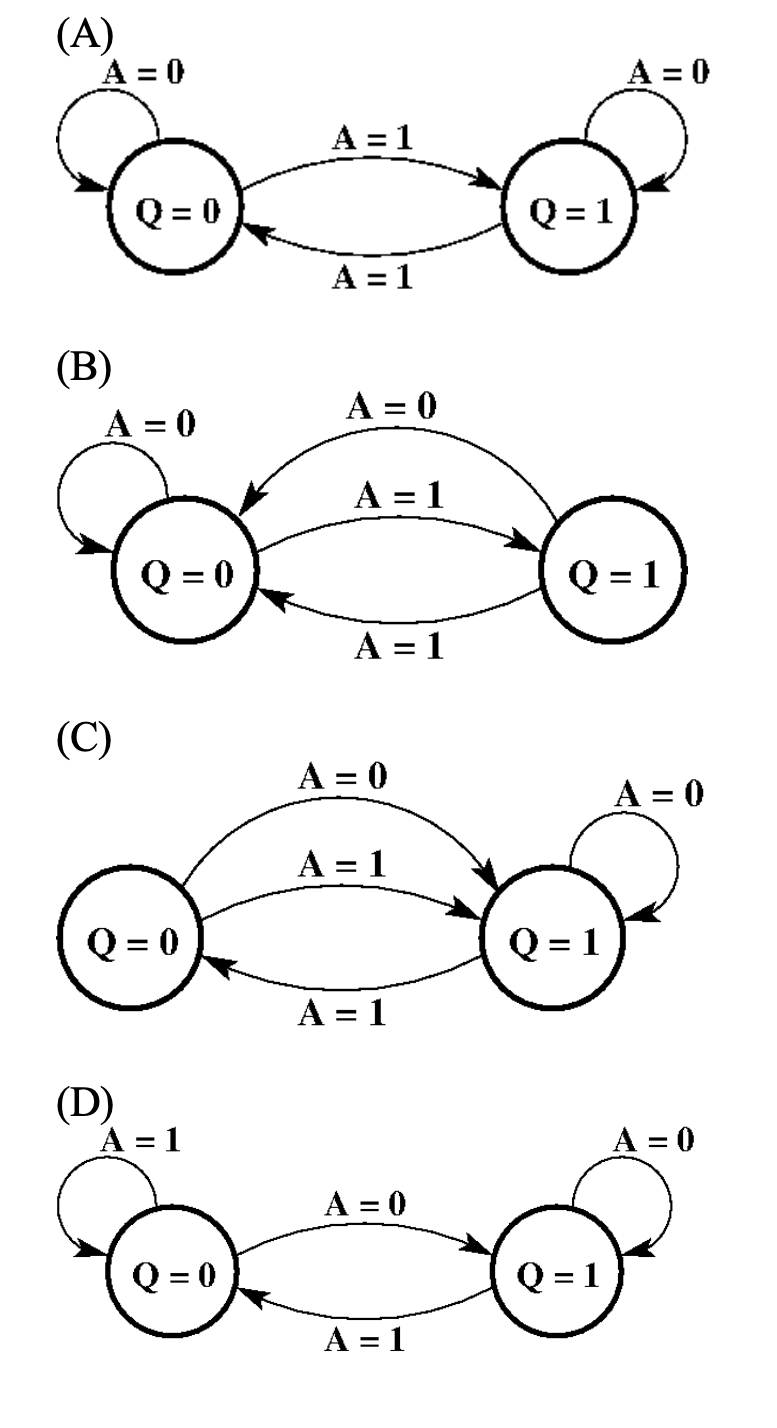
\includegraphics[scale=.33]{fig2.PNG}}
	
	\label{fig2.PNG}
\end{figure}
\end{frame}
%
\section{Answer}
\frametitle{Answer}
\subsection{multiplexer}
\begin{frame}{multiplexer}
 \begin{figure}[!ht]
\centerline{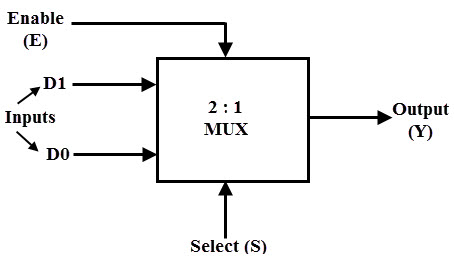
\includegraphics[scale=.34]{multiplexer.jpg}}
	
	\label{multiplexer.jpg}
	
\end{figure}
There are total 5 types of multiplexer it varies in no of inputs
\break 
It is also known as \underline{Data Selector}
\break
The relation between selctor and no of inputs is (s = log_2 n)

if the selector(A) is 0 then the output will be 1 similarly the other
therefore, output y can be 1 or 0
\break
\end{frame}
\subsection{D flip flop}
%
\begin{frame}{D flip flop}
    \begin{figure}[!ht]
\centerline{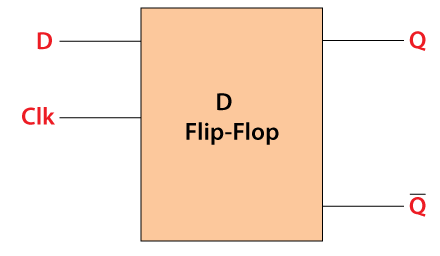
\includegraphics[scale=.34]{flipflop.png}}
	
	\label{filpflop.png}
	
\end{figure}
%
The memory element in a sequential circuit is called as a flip flop
\break
from the question D = \overline{Q.y}
\break
\end{frame}
\frametitle{Truth table}
  \subsection{truth table}
  
    \begin{figure}[!ht]
\centerline{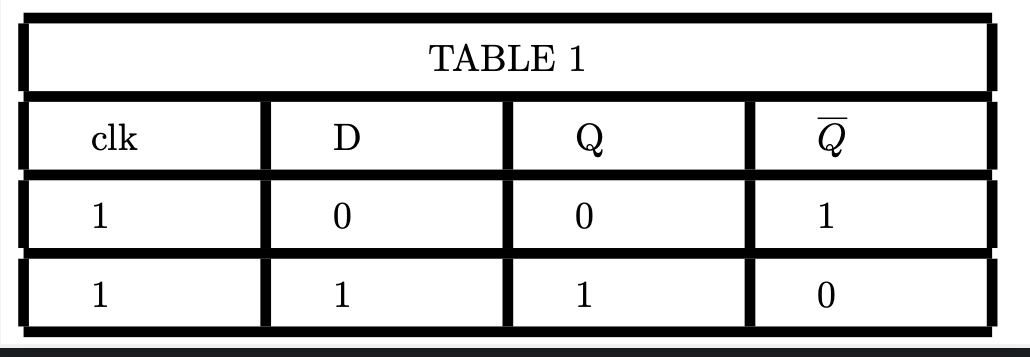
\includegraphics[scale=0.5]{table.png}}
	
	\label{table.png}

  from the truth table the total possible outputs for Q = 0,1
  \break
 1) so let us take Q = 0  when the selector A = 0,
    y = 1
    \break
    D = \overline{Q}+\overline{y}
    \break
    = 1 + 0 = 1
    
     when the  selctor(A) is 1 then y = 0
    \break
     then D = 1 + 1 =1
     \break 
2) now take Q = 1
     when selector A = 0, output y = 1
     \break
     then D = 0 + 0 = 0
     \break
     when selector A = 1, output y = 0
     \break
     then D = 0 + 1 = 1
     \break
  
 \end{frame}
 \begin{frame}{state transition diagram}
 \frametitle{state transition}
 \subsection{state transition diagram}
 \begin{frame}{state transition diagram}
   \begin{figure}[!ht]
\centerline{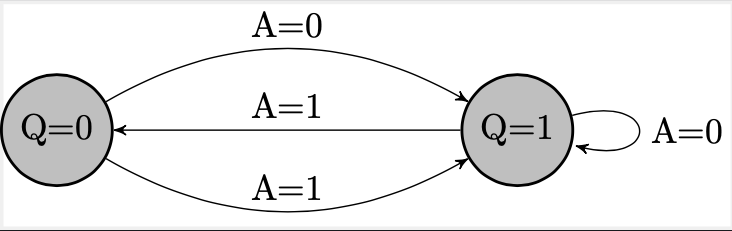
\includegraphics[scale=0.5]{state transition.png}}
	
	\label{state transition.png}
	\end{figure}
  the diagram itself explains, the Q = 0 state opens door and the transition goes to state Q = 1
  \break
  similarly  the transition goes from state Q = 1 to Q = 0 when the transition condition is A = 1.
\end{frame}
\begin{frame}
    \centering
    \textit{Thank you.}
\end{frame}

\end{document}
